% Options for packages loaded elsewhere
\PassOptionsToPackage{unicode}{hyperref}
\PassOptionsToPackage{hyphens}{url}
%
\documentclass[
]{article}
\title{The Impact of the 2011 Tōhoku tsunami on albatross in Hawaii}
\author{true}
\date{2022-01-09}

\usepackage{amsmath,amssymb}
\usepackage{lmodern}
\usepackage{iftex}
\ifPDFTeX
  \usepackage[T1]{fontenc}
  \usepackage[utf8]{inputenc}
  \usepackage{textcomp} % provide euro and other symbols
\else % if luatex or xetex
  \usepackage{unicode-math}
  \defaultfontfeatures{Scale=MatchLowercase}
  \defaultfontfeatures[\rmfamily]{Ligatures=TeX,Scale=1}
\fi
% Use upquote if available, for straight quotes in verbatim environments
\IfFileExists{upquote.sty}{\usepackage{upquote}}{}
\IfFileExists{microtype.sty}{% use microtype if available
  \usepackage[]{microtype}
  \UseMicrotypeSet[protrusion]{basicmath} % disable protrusion for tt fonts
}{}
\makeatletter
\@ifundefined{KOMAClassName}{% if non-KOMA class
  \IfFileExists{parskip.sty}{%
    \usepackage{parskip}
  }{% else
    \setlength{\parindent}{0pt}
    \setlength{\parskip}{6pt plus 2pt minus 1pt}}
}{% if KOMA class
  \KOMAoptions{parskip=half}}
\makeatother
\usepackage{xcolor}
\IfFileExists{xurl.sty}{\usepackage{xurl}}{} % add URL line breaks if available
\IfFileExists{bookmark.sty}{\usepackage{bookmark}}{\usepackage{hyperref}}
\hypersetup{
  pdftitle={The Impact of the 2011 Tōhoku tsunami on albatross in Hawaii},
  hidelinks,
  pdfcreator={LaTeX via pandoc}}
\urlstyle{same} % disable monospaced font for URLs
\usepackage[margin=1in]{geometry}
\usepackage{color}
\usepackage{fancyvrb}
\newcommand{\VerbBar}{|}
\newcommand{\VERB}{\Verb[commandchars=\\\{\}]}
\DefineVerbatimEnvironment{Highlighting}{Verbatim}{commandchars=\\\{\}}
% Add ',fontsize=\small' for more characters per line
\usepackage{framed}
\definecolor{shadecolor}{RGB}{248,248,248}
\newenvironment{Shaded}{\begin{snugshade}}{\end{snugshade}}
\newcommand{\AlertTok}[1]{\textcolor[rgb]{0.94,0.16,0.16}{#1}}
\newcommand{\AnnotationTok}[1]{\textcolor[rgb]{0.56,0.35,0.01}{\textbf{\textit{#1}}}}
\newcommand{\AttributeTok}[1]{\textcolor[rgb]{0.77,0.63,0.00}{#1}}
\newcommand{\BaseNTok}[1]{\textcolor[rgb]{0.00,0.00,0.81}{#1}}
\newcommand{\BuiltInTok}[1]{#1}
\newcommand{\CharTok}[1]{\textcolor[rgb]{0.31,0.60,0.02}{#1}}
\newcommand{\CommentTok}[1]{\textcolor[rgb]{0.56,0.35,0.01}{\textit{#1}}}
\newcommand{\CommentVarTok}[1]{\textcolor[rgb]{0.56,0.35,0.01}{\textbf{\textit{#1}}}}
\newcommand{\ConstantTok}[1]{\textcolor[rgb]{0.00,0.00,0.00}{#1}}
\newcommand{\ControlFlowTok}[1]{\textcolor[rgb]{0.13,0.29,0.53}{\textbf{#1}}}
\newcommand{\DataTypeTok}[1]{\textcolor[rgb]{0.13,0.29,0.53}{#1}}
\newcommand{\DecValTok}[1]{\textcolor[rgb]{0.00,0.00,0.81}{#1}}
\newcommand{\DocumentationTok}[1]{\textcolor[rgb]{0.56,0.35,0.01}{\textbf{\textit{#1}}}}
\newcommand{\ErrorTok}[1]{\textcolor[rgb]{0.64,0.00,0.00}{\textbf{#1}}}
\newcommand{\ExtensionTok}[1]{#1}
\newcommand{\FloatTok}[1]{\textcolor[rgb]{0.00,0.00,0.81}{#1}}
\newcommand{\FunctionTok}[1]{\textcolor[rgb]{0.00,0.00,0.00}{#1}}
\newcommand{\ImportTok}[1]{#1}
\newcommand{\InformationTok}[1]{\textcolor[rgb]{0.56,0.35,0.01}{\textbf{\textit{#1}}}}
\newcommand{\KeywordTok}[1]{\textcolor[rgb]{0.13,0.29,0.53}{\textbf{#1}}}
\newcommand{\NormalTok}[1]{#1}
\newcommand{\OperatorTok}[1]{\textcolor[rgb]{0.81,0.36,0.00}{\textbf{#1}}}
\newcommand{\OtherTok}[1]{\textcolor[rgb]{0.56,0.35,0.01}{#1}}
\newcommand{\PreprocessorTok}[1]{\textcolor[rgb]{0.56,0.35,0.01}{\textit{#1}}}
\newcommand{\RegionMarkerTok}[1]{#1}
\newcommand{\SpecialCharTok}[1]{\textcolor[rgb]{0.00,0.00,0.00}{#1}}
\newcommand{\SpecialStringTok}[1]{\textcolor[rgb]{0.31,0.60,0.02}{#1}}
\newcommand{\StringTok}[1]{\textcolor[rgb]{0.31,0.60,0.02}{#1}}
\newcommand{\VariableTok}[1]{\textcolor[rgb]{0.00,0.00,0.00}{#1}}
\newcommand{\VerbatimStringTok}[1]{\textcolor[rgb]{0.31,0.60,0.02}{#1}}
\newcommand{\WarningTok}[1]{\textcolor[rgb]{0.56,0.35,0.01}{\textbf{\textit{#1}}}}
\usepackage{graphicx}
\makeatletter
\def\maxwidth{\ifdim\Gin@nat@width>\linewidth\linewidth\else\Gin@nat@width\fi}
\def\maxheight{\ifdim\Gin@nat@height>\textheight\textheight\else\Gin@nat@height\fi}
\makeatother
% Scale images if necessary, so that they will not overflow the page
% margins by default, and it is still possible to overwrite the defaults
% using explicit options in \includegraphics[width, height, ...]{}
\setkeys{Gin}{width=\maxwidth,height=\maxheight,keepaspectratio}
% Set default figure placement to htbp
\makeatletter
\def\fps@figure{htbp}
\makeatother
\setlength{\emergencystretch}{3em} % prevent overfull lines
\providecommand{\tightlist}{%
  \setlength{\itemsep}{0pt}\setlength{\parskip}{0pt}}
\setcounter{secnumdepth}{-\maxdimen} % remove section numbering
\newlength{\cslhangindent}
\setlength{\cslhangindent}{1.5em}
\newlength{\csllabelwidth}
\setlength{\csllabelwidth}{3em}
\newlength{\cslentryspacingunit} % times entry-spacing
\setlength{\cslentryspacingunit}{\parskip}
\newenvironment{CSLReferences}[2] % #1 hanging-ident, #2 entry spacing
 {% don't indent paragraphs
  \setlength{\parindent}{0pt}
  % turn on hanging indent if param 1 is 1
  \ifodd #1
  \let\oldpar\par
  \def\par{\hangindent=\cslhangindent\oldpar}
  \fi
  % set entry spacing
  \setlength{\parskip}{#2\cslentryspacingunit}
 }%
 {}
\usepackage{calc}
\newcommand{\CSLBlock}[1]{#1\hfill\break}
\newcommand{\CSLLeftMargin}[1]{\parbox[t]{\csllabelwidth}{#1}}
\newcommand{\CSLRightInline}[1]{\parbox[t]{\linewidth - \csllabelwidth}{#1}\break}
\newcommand{\CSLIndent}[1]{\hspace{\cslhangindent}#1}
\usepackage{booktabs}
\usepackage{longtable}
\usepackage{array}
\usepackage{multirow}
\usepackage{wrapfig}
\usepackage{float}
\usepackage{colortbl}
\usepackage{pdflscape}
\usepackage{tabu}
\usepackage{threeparttable}
\usepackage{threeparttablex}
\usepackage[normalem]{ulem}
\usepackage{makecell}
\usepackage{xcolor}
\ifLuaTeX
  \usepackage{selnolig}  % disable illegal ligatures
\fi

\begin{document}
\maketitle

This is an image of Hōlanikū, also know as Kure Atoll, the northernmost
landmass in the Hawaiian archipelago. It is located at 28.3925° N,
178.2936° W and is within the Papahānaumokuākea National Marine
Monument. \emph{Image Credit: Kure Atoll Conservancy}

This statistical analysis was completed as an assignment for my Master's
program course, Environmental Data Science 222: Statistics for
Environmental Data Science.

\hypertarget{research-question}{%
\subsection{Research Question}\label{research-question}}

\emph{Were albatross populations impacted by the 2011 Tōhoku tsunami
event?}

Researchers estimated the Tōhoku tsunami flooded between 26\% - 52\% of
all Black-footed albatross nests and impacted more than 275,000
albatross nests throughout Papahānaumokuākea (Reynolds et al. 2017).
This post will attempt to analyze and quantify the impact of the Tōhoku
tsunami on two Hawaiian albatross species, the Laysan albatross and the
Black-footed albatross.

\hypertarget{background}{%
\subsection{Background}\label{background}}

The Hawaiian archipelago is home to thousands of albatrosses.
Albatrosses are an incredible bird species that have inspired authors,
the fashion industry, and birders across the globe. They live to be over
65 years old, have the largest wingspan of any bird, are monogamous
rearers, and have nest-site fidelity (meaning they return to the same
nest location every year). Three species of albatross breed in Hawaii,
the Laysan (\emph{Phoebastria immutabilis}), Black-footed
(\emph{Phoebastria nigripes}), and Short-tailed (\emph{Phoebastria
albatrus}) albatross. Laysan albatrosses are listed as near threatened
due to threats from climate change to their habitat and breeding grounds
and long-line fishing operations (Arata, Sievert, and Naughton 2009).
The IUCN Red List of Threatened Species assessed the Black-footed
albatross as near threatened in 2020 (List 2017). The Short-tailed
albatross almost went extinct in the early 1900s due to feather hunting
and is currently listed as an endangered species in the United States
(Alaska Region, n.d.).

\begin{Shaded}
\begin{Highlighting}[]
\FunctionTok{data.frame}\NormalTok{(}\StringTok{"Common\_name"} \OtherTok{=} \FunctionTok{c}\NormalTok{(}\StringTok{"Black{-}foot albatross"}\NormalTok{, }\StringTok{"Laysan albatross"}\NormalTok{, }\StringTok{"Short{-}tailed albatross"}\NormalTok{),}
           \StringTok{"Hawaiian\_name"} \OtherTok{=} \FunctionTok{c}\NormalTok{(}\StringTok{"Kaʻupu"}\NormalTok{, }\StringTok{"Mōlī"}\NormalTok{, }\StringTok{"Makalena or Kaʻupuakea"}\NormalTok{),}
           \StringTok{"Species\_code"} \OtherTok{=} \FunctionTok{c}\NormalTok{(}\StringTok{"BFAL"}\NormalTok{,}\StringTok{"LAAL"}\NormalTok{, }\StringTok{"STAL"}\NormalTok{),}
           \StringTok{"Scientific\_name"} \OtherTok{=} \FunctionTok{c}\NormalTok{(}\StringTok{"Phoebastria nigripes"}\NormalTok{, }\StringTok{"Phoebastria immutabilis"}\NormalTok{, }\StringTok{"Phoebastria albatrus"}\NormalTok{)) }\SpecialCharTok{\%\textgreater{}\%} 
  \FunctionTok{kable}\NormalTok{(}\AttributeTok{caption =} \StringTok{"Hawaiian Albatross Species Names"}\NormalTok{) }\SpecialCharTok{\%\textgreater{}\%}
  \FunctionTok{kable\_paper}\NormalTok{(}\AttributeTok{full\_width =} \ConstantTok{FALSE}\NormalTok{) }\SpecialCharTok{\%\textgreater{}\%}
  \FunctionTok{kable\_styling}\NormalTok{(}\AttributeTok{latex\_options =} \StringTok{"striped"}\NormalTok{,}
                \AttributeTok{font\_size =} \DecValTok{15}\NormalTok{) }\SpecialCharTok{\%\textgreater{}\%} 
  \FunctionTok{column\_spec}\NormalTok{(}\DecValTok{1}\NormalTok{, }\AttributeTok{bold =}\NormalTok{ T) }\SpecialCharTok{\%\textgreater{}\%}
  \FunctionTok{row\_spec}\NormalTok{(}\DecValTok{0}\NormalTok{, }\AttributeTok{bold =}\NormalTok{ T, }\AttributeTok{color =} \StringTok{"black"}\NormalTok{)}
\end{Highlighting}
\end{Shaded}

\begin{table}

\caption{\label{tab:unnamed-chunk-2}Hawaiian Albatross Species Names}
\centering
\fontsize{15}{17}\selectfont
\begin{tabular}[t]{>{}l|l|l|l}
\hline
\textcolor{black}{\textbf{Common\_name}} & \textcolor{black}{\textbf{Hawaiian\_name}} & \textcolor{black}{\textbf{Species\_code}} & \textcolor{black}{\textbf{Scientific\_name}}\\
\hline
\textbf{\cellcolor{gray!6}{Black-foot albatross}} & \cellcolor{gray!6}{Kaʻupu} & \cellcolor{gray!6}{BFAL} & \cellcolor{gray!6}{Phoebastria nigripes}\\
\hline
\textbf{Laysan albatross} & Mōlī & LAAL & Phoebastria immutabilis\\
\hline
\textbf{\cellcolor{gray!6}{Short-tailed albatross}} & \cellcolor{gray!6}{Makalena or Kaʻupuakea} & \cellcolor{gray!6}{STAL} & \cellcolor{gray!6}{Phoebastria albatrus}\\
\hline
\end{tabular}
\end{table}

Adult and juvenile Laysan and Black-footed albatross on the coral runway
of Hōlanikū (Kure Atoll). \emph{Image Credit: J. Parish}

Papahānaumokuākea, also known as the Northwestern Hawaiian Islands, are
comprised of atolls, reefs, and pinnacles, and are where 95\% of all
Black-footed albatross and 99\% of Laysan albatross nest (Arata,
Sievert, and Naughton 2009). These low-lying islands are at extreme risk
of inundation from tsunamis (Reynolds et al. 2017). On March 11, 2011, a
9.0 earthquake hit the Tōhoku region of Japan. The earthquake lasted
over 6 minutes, creating a tsunami that impacted coastal areas and
island nations throughout the Pacific region. Approximately 20,000
people lost their lives from the earthquake and resulting tsunami. The
tsunami also killed or injured thousands of marine and terrestrial
species. Many wildlife species found in the Papahānaumokuākea Marine
National Monument (PMNM) were impacted by the Tōhoku tsunami.

\emph{\textbf{Note}: The Short-tailed albatross was not included in this
analysis as there is only one breeding pair in Hawaii.}

\hypertarget{analysis-plan}{%
\subsection{Analysis Plan}\label{analysis-plan}}

This statistical analysis will be testing the hypothesis if the Tōhoku
tsunami impacted albatross populations in Hawaii. The table below
outlines the phases of the analysis.

\[H_{0}: There\ was\ no\ impact\ of\ the\ Tōhoku\ tsunami\ on\ albatross\ populations\ in\ Hawaii.\]
\[H_{1}: There\ was\ an\ impact\ of\ the\ Tōhoku\ tsunami\ on\ albatross\ populations\ in\ Hawaii.\]

\begin{Shaded}
\begin{Highlighting}[]
\FunctionTok{data.frame}\NormalTok{(}\StringTok{"Phase"} \OtherTok{=} \FunctionTok{c}\NormalTok{(}\DecValTok{1}\SpecialCharTok{:}\DecValTok{5}\NormalTok{),}
           \StringTok{"Description"} \OtherTok{=} \FunctionTok{c}\NormalTok{(}\StringTok{"Identify research question"}\NormalTok{,}
                             \StringTok{"Collect data"}\NormalTok{,}
                             \StringTok{"Visualize data"}\NormalTok{,}
                             \StringTok{"Conduct regression analysis"}\NormalTok{,}
                             \StringTok{"Conclusion \& Future Research"}\NormalTok{)) }\SpecialCharTok{\%\textgreater{}\%} 
  \FunctionTok{kable}\NormalTok{(}\AttributeTok{caption =} \StringTok{"Tōhoku Tsunami Impact Analysis Plan Outline"}\NormalTok{) }\SpecialCharTok{\%\textgreater{}\%}
  \FunctionTok{kable\_paper}\NormalTok{(}\AttributeTok{full\_width =} \ConstantTok{FALSE}\NormalTok{) }\SpecialCharTok{\%\textgreater{}\%}
  \FunctionTok{kable\_styling}\NormalTok{(}\AttributeTok{latex\_options =} \StringTok{"striped"}\NormalTok{,}
                \AttributeTok{font\_size =} \DecValTok{15}\NormalTok{) }\SpecialCharTok{\%\textgreater{}\%} 
  \FunctionTok{column\_spec}\NormalTok{(}\DecValTok{1}\NormalTok{, }\AttributeTok{bold =}\NormalTok{ T) }\SpecialCharTok{\%\textgreater{}\%}
  \FunctionTok{row\_spec}\NormalTok{(}\DecValTok{0}\NormalTok{, }\AttributeTok{bold =}\NormalTok{ T, }\AttributeTok{color =} \StringTok{"black"}\NormalTok{)}
\end{Highlighting}
\end{Shaded}

\begin{table}

\caption{\label{tab:unnamed-chunk-3}Tōhoku Tsunami Impact Analysis Plan Outline}
\centering
\fontsize{15}{17}\selectfont
\begin{tabular}[t]{>{}r|l}
\hline
\textcolor{black}{\textbf{Phase}} & \textcolor{black}{\textbf{Description}}\\
\hline
\textbf{\cellcolor{gray!6}{1}} & \cellcolor{gray!6}{Identify research question}\\
\hline
\textbf{2} & Collect data\\
\hline
\textbf{\cellcolor{gray!6}{3}} & \cellcolor{gray!6}{Visualize data}\\
\hline
\textbf{4} & Conduct regression analysis\\
\hline
\textbf{\cellcolor{gray!6}{5}} & \cellcolor{gray!6}{Conclusion \& Future Research}\\
\hline
\end{tabular}
\end{table}

\hypertarget{collect-data}{%
\subsection{Collect Data}\label{collect-data}}

After researching several data sources for albatross populations, I
retrieved banding data for both Laysan and Black-footed albatross from
the USGS Bird Banding Laboratory (BBL). The BBL has data on bird species
for the past 100 years. The data contains information about an
individual bird's sex, age, health condition, and coordinates where the
bird was banded. To access data from the BBL, it requires establishing
an account on the
\href{https://www.pwrc.usgs.gov/bbl/Bander_portal/login/main_login.php}{USGS
Bird Banding Lab Bander Portal website}. Once you submit a data request,
files will be available for download within 24 - 48 hours. I requested
data for Black-footed and Laysan albatrosses in Hawaii between the years
1996 and 2020.

Author and a colleague banding a juvenile Black-footed albatross.
\emph{Image Credit: E. Opie}

\begin{Shaded}
\begin{Highlighting}[]
\CommentTok{\# read in banding data}
\NormalTok{albie\_band }\OtherTok{\textless{}{-}} \FunctionTok{read\_csv}\NormalTok{(}\FunctionTok{here}\NormalTok{(}\StringTok{"\_posts"}\NormalTok{, }\StringTok{"2022{-}01{-}09{-}hawaii{-}albatross{-}tohoku{-}tsunami"}\NormalTok{, }\StringTok{"data"}\NormalTok{, }\StringTok{"laal\_bfal\_ca\_hi\_bbl2021.csv"}\NormalTok{)) }\CommentTok{\#both bfal and laal banding data for CA and HI}
\end{Highlighting}
\end{Shaded}

\hypertarget{visualize-data}{%
\subsection{Visualize Data}\label{visualize-data}}

Upon completion of data tidying and transformation, the next phase of
analysis is to visualize the data.

\hypertarget{distribution-map}{%
\paragraph{Distribution Map}\label{distribution-map}}

The initial visualization was to map the banding data on to a map of
Hawaii using the
\href{https://cran.r-project.org/web/packages/ggmap/readme/README.html}{ggmap()
package}. The banding data point distribution accurately reflects the
known species distribution of both species of albatross in Hawaii. The
only two main Hawaiian Islands where albatross nest are Kauai and Oahu.
This map shows most albatross populations reside with the PMNM.

\begin{Shaded}
\begin{Highlighting}[]
\NormalTok{albie\_map }\OtherTok{\textless{}{-}} \FunctionTok{ggmap}\NormalTok{(hawaii\_map) }\SpecialCharTok{+}
  \FunctionTok{geom\_point}\NormalTok{(}\FunctionTok{aes}\NormalTok{(}\AttributeTok{x =}\NormalTok{ lon\_dd, }\AttributeTok{y =}\NormalTok{ lat\_dd, }\AttributeTok{color =}\NormalTok{ species\_name),}
             \AttributeTok{data =}\NormalTok{ albie\_band,}
             \AttributeTok{size =} \FloatTok{0.5}\NormalTok{,}
             \AttributeTok{alpha =} \FloatTok{0.25}\NormalTok{) }\SpecialCharTok{+}
  \FunctionTok{scale\_color\_manual}\NormalTok{(}\AttributeTok{name =} \StringTok{"Albatross species"}\NormalTok{,}
                     \AttributeTok{values =} \FunctionTok{c}\NormalTok{(}\StringTok{"\#9E7E8C"}\NormalTok{, }\StringTok{"\#39ACB1"}\NormalTok{),}
                     \AttributeTok{labels =} \FunctionTok{c}\NormalTok{(}\StringTok{"Black{-}footed Albatross"}\NormalTok{, }\StringTok{"Laysan Albatross"}\NormalTok{),}
                     \AttributeTok{guide =} \FunctionTok{guide\_legend}\NormalTok{(}\AttributeTok{override.aes =} \FunctionTok{list}\NormalTok{(}\AttributeTok{size =} \DecValTok{3}\NormalTok{, }\AttributeTok{alpha =} \DecValTok{1}\NormalTok{))) }\SpecialCharTok{+}
  \FunctionTok{annotate}\NormalTok{(}\StringTok{"rect"}\NormalTok{, }\AttributeTok{xmin =} \SpecialCharTok{{-}}\FloatTok{162.13}\NormalTok{, }\AttributeTok{xmax =} \SpecialCharTok{{-}}\FloatTok{161.78}\NormalTok{, }\AttributeTok{ymin =} \FloatTok{22.94}\NormalTok{, }\AttributeTok{ymax =} \FloatTok{23.22}\NormalTok{, }
           \AttributeTok{color =} \StringTok{"\#728A72"}\NormalTok{, }\AttributeTok{fill =} \StringTok{"white"}\NormalTok{, }\AttributeTok{alpha =} \FloatTok{0.2}\NormalTok{) }\SpecialCharTok{+}
  \FunctionTok{annotate}\NormalTok{(}\StringTok{\textquotesingle{}text\textquotesingle{}}\NormalTok{, }\AttributeTok{x =} \SpecialCharTok{{-}}\FloatTok{161.7}\NormalTok{, }\AttributeTok{y =} \FloatTok{23.3}\NormalTok{, }
           \AttributeTok{label =} \StringTok{\textquotesingle{}Nihoa\textquotesingle{}}\NormalTok{, }\AttributeTok{color =} \StringTok{\textquotesingle{}black\textquotesingle{}}\NormalTok{, }\AttributeTok{size =} \FloatTok{2.3}\NormalTok{, }\AttributeTok{hjust =} \DecValTok{0}\NormalTok{) }\SpecialCharTok{+}
  \FunctionTok{annotate}\NormalTok{(}\StringTok{"rect"}\NormalTok{, }\AttributeTok{xmin =} \SpecialCharTok{{-}}\FloatTok{164.856}\NormalTok{, }\AttributeTok{xmax =} \SpecialCharTok{{-}}\FloatTok{164.55}\NormalTok{, }\AttributeTok{ymin =} \FloatTok{23.42}\NormalTok{, }\AttributeTok{ymax =} \FloatTok{23.74}\NormalTok{, }
           \AttributeTok{color =} \StringTok{"\#728A72"}\NormalTok{, }\AttributeTok{fill =} \StringTok{"white"}\NormalTok{, }\AttributeTok{alpha =} \FloatTok{0.2}\NormalTok{) }\SpecialCharTok{+}
  \FunctionTok{annotate}\NormalTok{(}\StringTok{\textquotesingle{}text\textquotesingle{}}\NormalTok{, }\AttributeTok{x =} \SpecialCharTok{{-}}\FloatTok{164.45}\NormalTok{, }\AttributeTok{y =} \FloatTok{23.8}\NormalTok{, }
           \AttributeTok{label =} \StringTok{\textquotesingle{}Mokumanamana\textquotesingle{}}\NormalTok{, }\AttributeTok{color =} \StringTok{\textquotesingle{}black\textquotesingle{}}\NormalTok{, }\AttributeTok{size =} \FloatTok{2.3}\NormalTok{, }\AttributeTok{hjust =} \DecValTok{0}\NormalTok{) }\SpecialCharTok{+}
  \FunctionTok{annotate}\NormalTok{(}\StringTok{"rect"}\NormalTok{, }\AttributeTok{xmin =} \SpecialCharTok{{-}}\FloatTok{166.54}\NormalTok{, }\AttributeTok{xmax =} \SpecialCharTok{{-}}\FloatTok{165.88}\NormalTok{, }\AttributeTok{ymin =} \FloatTok{23.45}\NormalTok{, }\AttributeTok{ymax =} \FloatTok{24.11}\NormalTok{, }
           \AttributeTok{color =} \StringTok{"\#728A72"}\NormalTok{, }\AttributeTok{fill =} \StringTok{"white"}\NormalTok{, }\AttributeTok{alpha =} \FloatTok{0.0}\NormalTok{) }\SpecialCharTok{+}
  \FunctionTok{annotate}\NormalTok{(}\StringTok{\textquotesingle{}text\textquotesingle{}}\NormalTok{, }\AttributeTok{x =} \SpecialCharTok{{-}}\FloatTok{166.54}\NormalTok{, }\AttributeTok{y =} \FloatTok{24.3}\NormalTok{, }
           \AttributeTok{label =} \StringTok{\textquotesingle{}Lalo\textquotesingle{}}\NormalTok{, }\AttributeTok{color =} \StringTok{\textquotesingle{}black\textquotesingle{}}\NormalTok{, }\AttributeTok{size =} \FloatTok{2.3}\NormalTok{, }\AttributeTok{hjust =} \DecValTok{0}\NormalTok{) }\SpecialCharTok{+}
  \FunctionTok{annotate}\NormalTok{(}\StringTok{"rect"}\NormalTok{, }\AttributeTok{xmin =} \SpecialCharTok{{-}}\FloatTok{168.19}\NormalTok{, }\AttributeTok{xmax =} \SpecialCharTok{{-}}\FloatTok{167.83}\NormalTok{, }\AttributeTok{ymin =} \FloatTok{24.82}\NormalTok{, }\AttributeTok{ymax =} \FloatTok{25.16}\NormalTok{, }
           \AttributeTok{color =} \StringTok{"\#728A72"}\NormalTok{, }\AttributeTok{fill =} \StringTok{"white"}\NormalTok{, }\AttributeTok{alpha =} \FloatTok{0.2}\NormalTok{) }\SpecialCharTok{+}
  \FunctionTok{annotate}\NormalTok{(}\StringTok{\textquotesingle{}text\textquotesingle{}}\NormalTok{, }\AttributeTok{x =} \SpecialCharTok{{-}}\FloatTok{167.8}\NormalTok{, }\AttributeTok{y =} \FloatTok{25.3}\NormalTok{, }
           \AttributeTok{label =} \StringTok{\textquotesingle{}Onunui\textquotesingle{}}\NormalTok{, }\AttributeTok{color =} \StringTok{\textquotesingle{}black\textquotesingle{}}\NormalTok{, }\AttributeTok{size =} \FloatTok{2.3}\NormalTok{, }\AttributeTok{hjust =} \DecValTok{0}\NormalTok{) }\SpecialCharTok{+}
  \FunctionTok{annotate}\NormalTok{(}\StringTok{"rect"}\NormalTok{, }\AttributeTok{xmin =} \SpecialCharTok{{-}}\FloatTok{170.78}\NormalTok{, }\AttributeTok{xmax =} \SpecialCharTok{{-}}\FloatTok{170.46}\NormalTok{, }\AttributeTok{ymin =} \FloatTok{25.33}\NormalTok{, }\AttributeTok{ymax =} \FloatTok{25.68}\NormalTok{, }
           \AttributeTok{color =} \StringTok{"\#728A72"}\NormalTok{, }\AttributeTok{fill =} \StringTok{"white"}\NormalTok{, }\AttributeTok{alpha =} \FloatTok{0.2}\NormalTok{) }\SpecialCharTok{+}
  \FunctionTok{annotate}\NormalTok{(}\StringTok{\textquotesingle{}text\textquotesingle{}}\NormalTok{, }\AttributeTok{x =} \SpecialCharTok{{-}}\FloatTok{170.39}\NormalTok{, }\AttributeTok{y =} \FloatTok{25.8}\NormalTok{, }
           \AttributeTok{label =} \StringTok{\textquotesingle{}Kamokuokamohoalii\textquotesingle{}}\NormalTok{, }\AttributeTok{color =} \StringTok{\textquotesingle{}black\textquotesingle{}}\NormalTok{, }\AttributeTok{size =} \FloatTok{2.3}\NormalTok{, }\AttributeTok{hjust =} \DecValTok{0}\NormalTok{) }\SpecialCharTok{+}
  \FunctionTok{annotate}\NormalTok{(}\StringTok{"rect"}\NormalTok{, }\AttributeTok{xmin =} \SpecialCharTok{{-}}\FloatTok{171.95}\NormalTok{, }\AttributeTok{xmax =} \SpecialCharTok{{-}}\FloatTok{171.45}\NormalTok{, }\AttributeTok{ymin =} \FloatTok{25.53}\NormalTok{, }\AttributeTok{ymax =} \DecValTok{26}\NormalTok{, }
           \AttributeTok{color =} \StringTok{"\#728A72"}\NormalTok{, }\AttributeTok{fill =} \StringTok{"white"}\NormalTok{, }\AttributeTok{alpha =} \FloatTok{0.0}\NormalTok{) }\SpecialCharTok{+}
  \FunctionTok{annotate}\NormalTok{(}\StringTok{\textquotesingle{}text\textquotesingle{}}\NormalTok{, }\AttributeTok{x =} \SpecialCharTok{{-}}\DecValTok{172}\NormalTok{, }\AttributeTok{y =} \FloatTok{26.2}\NormalTok{, }
           \AttributeTok{label =} \StringTok{\textquotesingle{}Kamole\textquotesingle{}}\NormalTok{, }\AttributeTok{color =} \StringTok{\textquotesingle{}black\textquotesingle{}}\NormalTok{, }\AttributeTok{size =} \FloatTok{2.3}\NormalTok{, }\AttributeTok{hjust =} \DecValTok{0}\NormalTok{) }\SpecialCharTok{+}
  \FunctionTok{annotate}\NormalTok{(}\StringTok{"rect"}\NormalTok{, }\AttributeTok{xmin =} \SpecialCharTok{{-}}\FloatTok{174.21}\NormalTok{, }\AttributeTok{xmax =} \SpecialCharTok{{-}}\FloatTok{173.8}\NormalTok{, }\AttributeTok{ymin =} \FloatTok{25.84}\NormalTok{, }\AttributeTok{ymax =} \FloatTok{26.24}\NormalTok{, }
           \AttributeTok{color =} \StringTok{"\#728A72"}\NormalTok{, }\AttributeTok{fill =} \StringTok{"white"}\NormalTok{, }\AttributeTok{alpha =} \FloatTok{0.2}\NormalTok{) }\SpecialCharTok{+}
  \FunctionTok{annotate}\NormalTok{(}\StringTok{\textquotesingle{}text\textquotesingle{}}\NormalTok{, }\AttributeTok{x =} \SpecialCharTok{{-}}\FloatTok{173.85}\NormalTok{, }\AttributeTok{y =} \FloatTok{26.5}\NormalTok{, }
           \AttributeTok{label =} \StringTok{\textquotesingle{}Kapou\textquotesingle{}}\NormalTok{, }\AttributeTok{color =} \StringTok{\textquotesingle{}black\textquotesingle{}}\NormalTok{, }\AttributeTok{size =} \FloatTok{2.3}\NormalTok{, }\AttributeTok{hjust =} \DecValTok{0}\NormalTok{) }\SpecialCharTok{+}
  \FunctionTok{annotate}\NormalTok{(}\StringTok{"rect"}\NormalTok{, }\AttributeTok{xmin =} \SpecialCharTok{{-}}\FloatTok{175.47}\NormalTok{, }\AttributeTok{xmax =} \SpecialCharTok{{-}}\FloatTok{174.9}\NormalTok{, }\AttributeTok{ymin =} \FloatTok{27.22}\NormalTok{, }\AttributeTok{ymax =} \FloatTok{27.61}\NormalTok{, }
           \AttributeTok{color =} \StringTok{"\#728A72"}\NormalTok{, }\AttributeTok{fill =} \StringTok{"white"}\NormalTok{, }\AttributeTok{alpha =} \FloatTok{0.2}\NormalTok{) }\SpecialCharTok{+}
  \FunctionTok{annotate}\NormalTok{(}\StringTok{\textquotesingle{}text\textquotesingle{}}\NormalTok{, }\AttributeTok{x =} \SpecialCharTok{{-}}\FloatTok{174.8}\NormalTok{, }\AttributeTok{y =} \FloatTok{27.7}\NormalTok{, }
           \AttributeTok{label =} \StringTok{\textquotesingle{}Kamole\textquotesingle{}}\NormalTok{, }\AttributeTok{color =} \StringTok{\textquotesingle{}black\textquotesingle{}}\NormalTok{, }\AttributeTok{size =} \FloatTok{2.3}\NormalTok{, }\AttributeTok{hjust =} \DecValTok{0}\NormalTok{) }\SpecialCharTok{+}
  \FunctionTok{annotate}\NormalTok{(}\StringTok{"rect"}\NormalTok{, }\AttributeTok{xmin =} \SpecialCharTok{{-}}\FloatTok{176.16}\NormalTok{, }\AttributeTok{xmax =} \SpecialCharTok{{-}}\FloatTok{175.53}\NormalTok{, }\AttributeTok{ymin =} \FloatTok{27.57}\NormalTok{, }\AttributeTok{ymax =} \FloatTok{28.14}\NormalTok{, }
           \AttributeTok{color =} \StringTok{"\#728A72"}\NormalTok{, }\AttributeTok{fill =} \StringTok{"white"}\NormalTok{, }\AttributeTok{alpha =} \FloatTok{0.0}\NormalTok{) }\SpecialCharTok{+}
  \FunctionTok{annotate}\NormalTok{(}\StringTok{\textquotesingle{}text\textquotesingle{}}\NormalTok{, }\AttributeTok{x =} \SpecialCharTok{{-}}\FloatTok{175.97}\NormalTok{, }\AttributeTok{y =} \FloatTok{28.35}\NormalTok{, }
           \AttributeTok{label =} \StringTok{\textquotesingle{}Kuaihelani\textquotesingle{}}\NormalTok{, }\AttributeTok{color =} \StringTok{\textquotesingle{}black\textquotesingle{}}\NormalTok{, }\AttributeTok{size =} \FloatTok{2.3}\NormalTok{, }\AttributeTok{hjust =} \DecValTok{0}\NormalTok{) }\SpecialCharTok{+}
  \FunctionTok{annotate}\NormalTok{(}\StringTok{"rect"}\NormalTok{, }\AttributeTok{xmin =} \SpecialCharTok{{-}}\FloatTok{177.19}\NormalTok{, }\AttributeTok{xmax =} \SpecialCharTok{{-}}\FloatTok{177.6}\NormalTok{, }\AttributeTok{ymin =} \FloatTok{28.1}\NormalTok{, }\AttributeTok{ymax =} \FloatTok{28.4}\NormalTok{, }
           \AttributeTok{color =} \StringTok{"\#728A72"}\NormalTok{, }\AttributeTok{fill =} \StringTok{"white"}\NormalTok{, }\AttributeTok{alpha =} \FloatTok{0.0}\NormalTok{) }\SpecialCharTok{+}
  \FunctionTok{annotate}\NormalTok{(}\StringTok{\textquotesingle{}text\textquotesingle{}}\NormalTok{, }\AttributeTok{x =} \SpecialCharTok{{-}}\FloatTok{177.55}\NormalTok{, }\AttributeTok{y =} \FloatTok{28.65}\NormalTok{, }
           \AttributeTok{label =} \StringTok{\textquotesingle{}Holaniku\textquotesingle{}}\NormalTok{, }\AttributeTok{color =} \StringTok{\textquotesingle{}black\textquotesingle{}}\NormalTok{, }\AttributeTok{size =} \FloatTok{2.3}\NormalTok{, }\AttributeTok{hjust =} \DecValTok{0}\NormalTok{) }\SpecialCharTok{+}
  \FunctionTok{annotate}\NormalTok{(}\StringTok{\textquotesingle{}text\textquotesingle{}}\NormalTok{, }\AttributeTok{x =} \SpecialCharTok{{-}}\FloatTok{177.5}\NormalTok{, }\AttributeTok{y =} \FloatTok{19.5}\NormalTok{, }
           \AttributeTok{label =} \StringTok{\textquotesingle{}Created: 2021 J. Parish}\SpecialCharTok{\textbackslash{}n}\StringTok{Data Source: USGS Bird Banding Lab\textquotesingle{}}\NormalTok{, }
           \AttributeTok{color =} \StringTok{\textquotesingle{}black\textquotesingle{}}\NormalTok{, }\AttributeTok{size =} \FloatTok{1.5}\NormalTok{, }\AttributeTok{hjust =} \DecValTok{0}\NormalTok{) }\SpecialCharTok{+}
  \FunctionTok{labs}\NormalTok{(}\AttributeTok{title =} \StringTok{"Figure 1: Banded Albatross Species in the Hawaiian Archipelago"}\NormalTok{,}
        \AttributeTok{subtitle =} \StringTok{"1996 {-} 2020"}\NormalTok{,}
        \AttributeTok{x =} \StringTok{"Longitude"}\NormalTok{,}
        \AttributeTok{y =} \StringTok{"Latitude"}\NormalTok{) }\SpecialCharTok{+}
  \FunctionTok{theme}\NormalTok{(}\AttributeTok{legend.title =} \FunctionTok{element\_text}\NormalTok{(}\AttributeTok{size=}\DecValTok{12}\NormalTok{, }\AttributeTok{color =} \StringTok{"black"}\NormalTok{, }\AttributeTok{face=}\StringTok{"bold"}\NormalTok{),}
           \AttributeTok{legend.justification=}\FunctionTok{c}\NormalTok{(}\DecValTok{0}\NormalTok{,}\DecValTok{1}\NormalTok{), }
           \AttributeTok{legend.position=}\FunctionTok{c}\NormalTok{(}\FloatTok{0.72}\NormalTok{, }\FloatTok{0.98}\NormalTok{),}
           \AttributeTok{legend.background =} \FunctionTok{element\_blank}\NormalTok{(),}
           \AttributeTok{legend.key =} \FunctionTok{element\_blank}\NormalTok{())}
\NormalTok{albie\_map}
\end{Highlighting}
\end{Shaded}

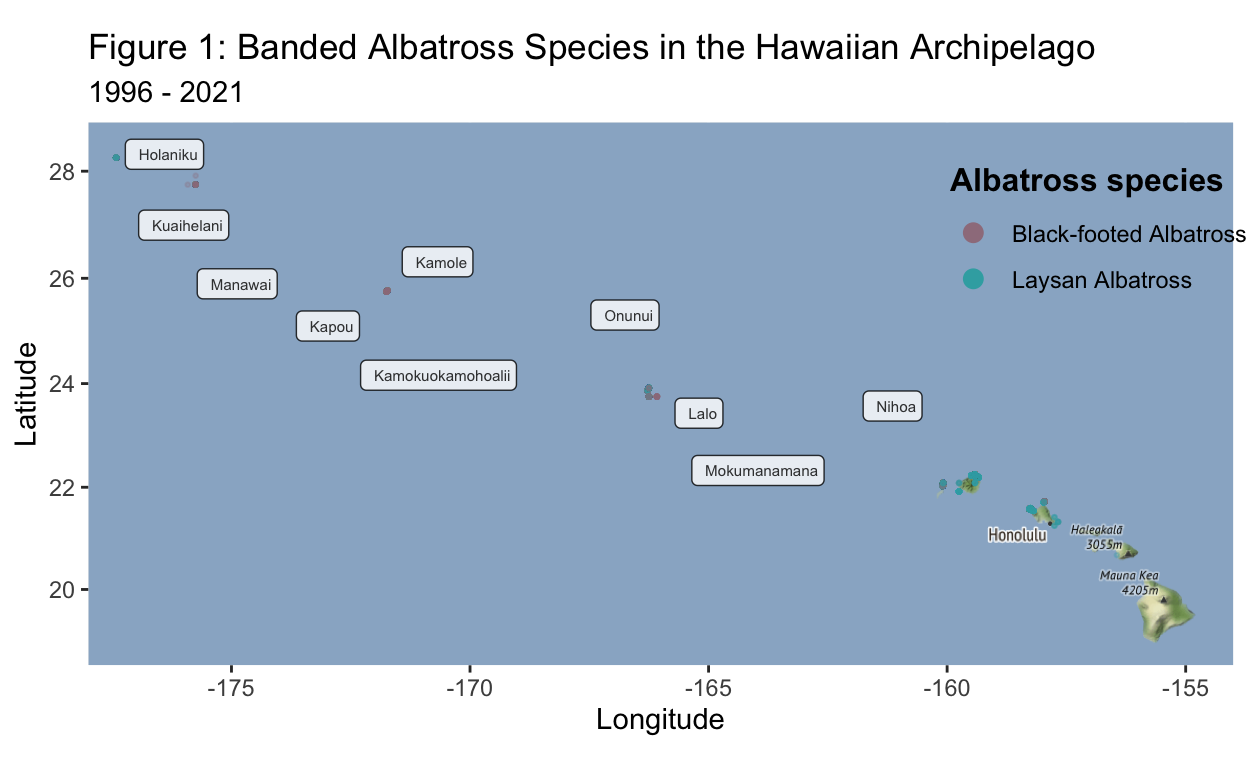
\includegraphics{hi_albatross_tokohu_tsunami_files/figure-latex/create albatross map-1.pdf}

\begin{Shaded}
\begin{Highlighting}[]
\NormalTok{band\_count }\OtherTok{\textless{}{-}}\NormalTok{ albie\_band }\SpecialCharTok{\%\textgreater{}\%} 
  \FunctionTok{group\_by}\NormalTok{(species, year) }\SpecialCharTok{\%\textgreater{}\%} 
  \FunctionTok{summarise}\NormalTok{(}\AttributeTok{total =} \FunctionTok{sum}\NormalTok{(count))}
\end{Highlighting}
\end{Shaded}

\hypertarget{scatterplot}{%
\paragraph{Scatterplot}\label{scatterplot}}

To conduct analysis on the albatross banding data, it is necessary to
create a total count of albatross banded for each year from 1996 to
2020. Once a total count was summed, I used a line and point plot to
visualize albatross count annually and added a line to indicate with the
Tōhoku tsunami occurred (2011). This plot does suggest that there may be
a negative effect from the Tōhoku tsunami on albatross populations as
the counts drop significantly after 2011. It also shows that the number
of banded Black-footed albatrosses declined more than Laysan albatrosses
after the tsunami. This trend may reflect the data that Reynolds et
al.~found as Black-footed albatrosses' nest along coastal areas whereas
Laysan albatrosses tend to nest more inland or at higher elevations on
islands (Reynolds et al. 2017).

\begin{Shaded}
\begin{Highlighting}[]
\CommentTok{\#plot banding count data}

\NormalTok{albie\_count\_plot }\OtherTok{\textless{}{-}} \FunctionTok{ggplot}\NormalTok{(band\_count, }\FunctionTok{aes}\NormalTok{(}\AttributeTok{x =}\NormalTok{ year, }\AttributeTok{y =}\NormalTok{ total, }\AttributeTok{group =}\NormalTok{ species)) }\SpecialCharTok{+}
  \FunctionTok{geom\_point}\NormalTok{(}\FunctionTok{aes}\NormalTok{(}\AttributeTok{color =}\NormalTok{ species,}
                 \AttributeTok{shape =}\NormalTok{ species)) }\SpecialCharTok{+}
  \FunctionTok{geom\_line}\NormalTok{(}\FunctionTok{aes}\NormalTok{(}\AttributeTok{color =}\NormalTok{ species)) }\SpecialCharTok{+}
  \FunctionTok{scale\_color\_manual}\NormalTok{(}\AttributeTok{name =} \StringTok{"Albatross species"}\NormalTok{,}
                     \AttributeTok{values =} \FunctionTok{c}\NormalTok{(}\StringTok{"\#9E7E8C"}\NormalTok{, }\StringTok{"\#39ACB1"}\NormalTok{),}
                     \AttributeTok{labels =} \FunctionTok{c}\NormalTok{(}\StringTok{"Black{-}footed Albatross (BFAL)"}\NormalTok{, }\StringTok{"Laysan Albatross (LAAL)"}\NormalTok{),}
                     \AttributeTok{guide =} \FunctionTok{guide\_legend}\NormalTok{(}\AttributeTok{override.aes =} \FunctionTok{list}\NormalTok{(}\AttributeTok{shape =} \FunctionTok{c}\NormalTok{(}\DecValTok{19}\NormalTok{, }\DecValTok{17}\NormalTok{)))) }\SpecialCharTok{+}
  \FunctionTok{geom\_vline}\NormalTok{(}\AttributeTok{xintercept =} \DecValTok{2011}\NormalTok{,}
             \AttributeTok{linetype =} \StringTok{"solid"}\NormalTok{,}
             \AttributeTok{color =} \StringTok{"goldenrod1"}\NormalTok{,}
             \AttributeTok{size =} \DecValTok{2}\NormalTok{) }\SpecialCharTok{+}
  \FunctionTok{guides}\NormalTok{(}\AttributeTok{shape =} \ConstantTok{FALSE}\NormalTok{) }\SpecialCharTok{+}
  \FunctionTok{annotate}\NormalTok{(}\StringTok{"text"}\NormalTok{,}
           \AttributeTok{label =} \StringTok{"Tōhoku tsunami"}\NormalTok{,}
           \AttributeTok{x =} \DecValTok{2014}\NormalTok{,}
           \AttributeTok{y =} \DecValTok{4700}\NormalTok{,}
           \AttributeTok{color =} \StringTok{"black"}\NormalTok{,}
           \AttributeTok{size =} \DecValTok{4}\NormalTok{) }\SpecialCharTok{+}
  \FunctionTok{labs}\NormalTok{(}\AttributeTok{title =} \StringTok{"Figure 2: Hawaii Albatross Count Based On Band Data"}\NormalTok{,}
       \AttributeTok{subtitle =} \StringTok{"Data source: USGS Bird Banding Lab"}\NormalTok{,}
       \AttributeTok{x =} \StringTok{"Year"}\NormalTok{,}
       \AttributeTok{y =} \StringTok{"Albatross Banded"}\NormalTok{,}
       \AttributeTok{color =} \StringTok{"Species"}\NormalTok{) }\SpecialCharTok{+}
  \FunctionTok{theme\_minimal}\NormalTok{() }\SpecialCharTok{+}
  \FunctionTok{theme}\NormalTok{(}\AttributeTok{legend.background =} \FunctionTok{element\_blank}\NormalTok{(),}
        \AttributeTok{legend.position =} \StringTok{"bottom"}\NormalTok{)  }
  
\NormalTok{albie\_count\_plot}
\end{Highlighting}
\end{Shaded}

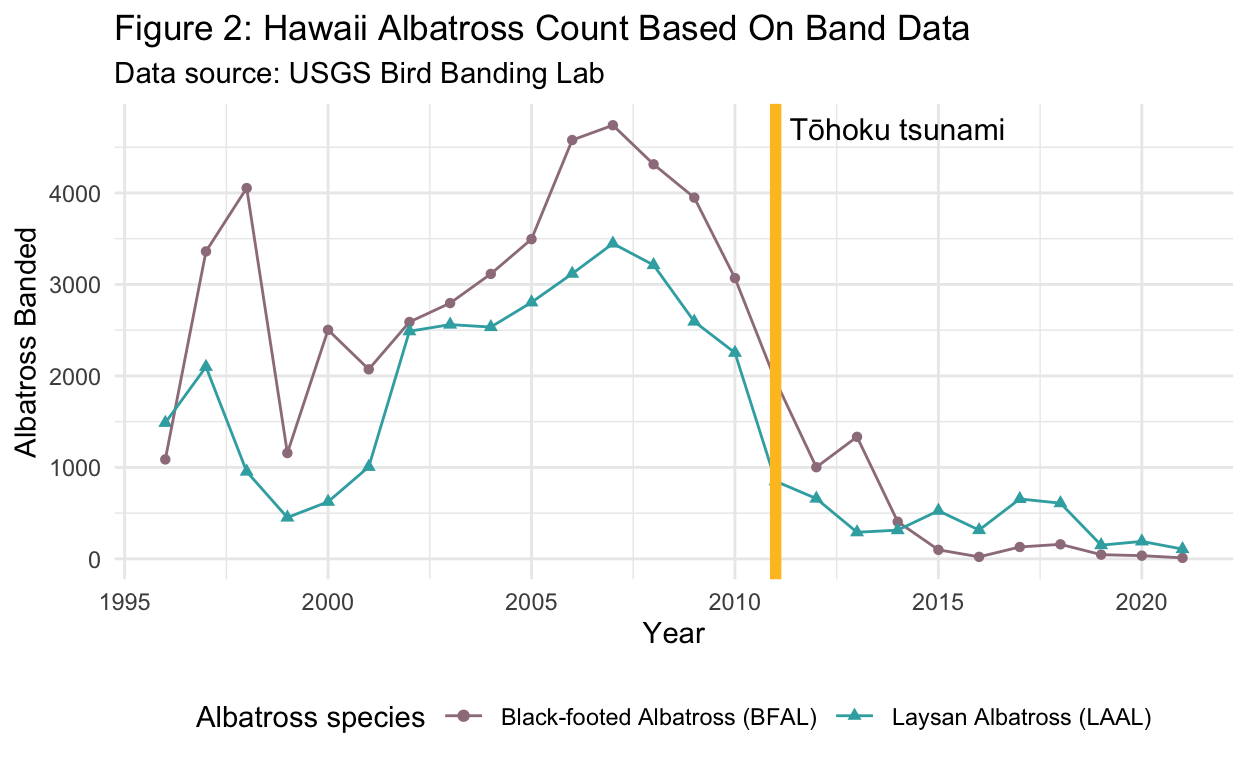
\includegraphics{hi_albatross_tokohu_tsunami_files/figure-latex/plot count by species-1.pdf}

\hypertarget{population-means}{%
\paragraph{Population Means}\label{population-means}}

I calculated the mean of banded albatross species between 1996 and 2020
as well as comparing the population means of each species pre- and
post-tsunami event. These means indicate that more black-foot albatross
is banded than Laysan albatross in Hawaii. This is an interesting data
point as the total Laysan albatross population is larger than the
Black-footed albatross population (VanderWerf 2012). The Laysan
albatross actually holds the honor of having the largest population of
all albatross species in the world (out of 21 species). Reviewing the
two population mean tables also indicated that the number of banded
albatrosses declined after the Tōhoku tsunami.

\begin{Shaded}
\begin{Highlighting}[]
\NormalTok{pop\_params\_table }\OtherTok{\textless{}{-}}\NormalTok{ knitr}\SpecialCharTok{::}\FunctionTok{kable}\NormalTok{(pop\_params\_summary,}
                                 \AttributeTok{digits =} \DecValTok{0}\NormalTok{,}
                                 \AttributeTok{col.names =} \FunctionTok{c}\NormalTok{(}\StringTok{\textquotesingle{}Albatross Species\textquotesingle{}}\NormalTok{, }\StringTok{\textquotesingle{}Population Mean\textquotesingle{}}\NormalTok{, }\StringTok{\textquotesingle{}Population Median\textquotesingle{}}\NormalTok{, }\StringTok{\textquotesingle{}Population Max\textquotesingle{}}\NormalTok{),}
                                 \AttributeTok{align =} \StringTok{"lccc"}\NormalTok{,}
                                 \AttributeTok{caption =} \StringTok{"Hawaii Albatross Population Summary 1996 {-} 2021"}\NormalTok{) }\SpecialCharTok{\%\textgreater{}\%}
  \FunctionTok{kable\_paper}\NormalTok{(}\AttributeTok{full\_width =} \ConstantTok{FALSE}\NormalTok{) }\SpecialCharTok{\%\textgreater{}\%}
  \FunctionTok{kable\_styling}\NormalTok{(}\AttributeTok{latex\_options =} \StringTok{"striped"}\NormalTok{,}
                \AttributeTok{font\_size =} \DecValTok{15}\NormalTok{) }\SpecialCharTok{\%\textgreater{}\%} 
  \FunctionTok{column\_spec}\NormalTok{(}\DecValTok{1}\NormalTok{, }\AttributeTok{bold =}\NormalTok{ T) }\SpecialCharTok{\%\textgreater{}\%}
  \FunctionTok{row\_spec}\NormalTok{(}\DecValTok{0}\NormalTok{, }\AttributeTok{bold =}\NormalTok{ T, }\AttributeTok{color =} \StringTok{"black"}\NormalTok{) }\CommentTok{\#\%\textgreater{}\% }
  \CommentTok{\# save\_kable(here("images/pop\_params.png"))}

\NormalTok{pop\_params\_table }
\end{Highlighting}
\end{Shaded}

\begin{table}

\caption{\label{tab:unnamed-chunk-11}Hawaii Albatross Population Summary 1996 - 2021}
\centering
\fontsize{15}{17}\selectfont
\begin{tabular}[t]{>{}l|c|c|c}
\hline
\textcolor{black}{\textbf{Albatross Species}} & \textcolor{black}{\textbf{Population Mean}} & \textcolor{black}{\textbf{Population Median}} & \textcolor{black}{\textbf{Population Max}}\\
\hline
\textbf{\cellcolor{gray!6}{BFAL}} & \cellcolor{gray!6}{2003} & \cellcolor{gray!6}{2008} & \cellcolor{gray!6}{4740}\\
\hline
\textbf{LAAL} & 1396 & 902 & 3447\\
\hline
\end{tabular}
\end{table}

\begin{Shaded}
\begin{Highlighting}[]
\NormalTok{pop\_mean\_table }\OtherTok{\textless{}{-}}\NormalTok{ knitr}\SpecialCharTok{::}\FunctionTok{kable}\NormalTok{(pop\_mean,}
                               \AttributeTok{col.names =} \FunctionTok{c}\NormalTok{(}\StringTok{\textquotesingle{}Species\textquotesingle{}}\NormalTok{, }\StringTok{\textquotesingle{}Pre\_Pop\_Mean\textquotesingle{}}\NormalTok{, }\StringTok{\textquotesingle{}Post\_Pop\_Mean\textquotesingle{}}\NormalTok{),}
                               \AttributeTok{caption =} \StringTok{"Hawaii Albatross Count Means Pre{-} \& Post{-} Tōhoku Tsunami"}\NormalTok{) }\SpecialCharTok{\%\textgreater{}\%} 
  \FunctionTok{kable\_classic}\NormalTok{(}\AttributeTok{full\_width =}\NormalTok{ F, }\AttributeTok{html\_font =} \StringTok{"Cambria"}\NormalTok{) }\CommentTok{\#\%\textgreater{}\% }
  \CommentTok{\# save\_kable(file = "images/albie\_mean\_pops.png",}
  \CommentTok{\#            zoom = 1.5)}

\NormalTok{pop\_mean\_table}
\end{Highlighting}
\end{Shaded}

\begin{table}

\caption{\label{tab:unnamed-chunk-15}Hawaii Albatross Count Means Pre- & Post- Tōhoku Tsunami}
\centering
\begin{tabular}[t]{l|r|r}
\hline
Species & Pre\_Pop\_Mean & Post\_Pop\_Mean\\
\hline
BFAL & 3627.11 & 517.8\\
\hline
LAAL & 2778.89 & 455.9\\
\hline
\end{tabular}
\end{table}

\hypertarget{conduct-and-interpret-regression-analysis}{%
\subsection{Conduct and Interpret Regression
Analysis}\label{conduct-and-interpret-regression-analysis}}

To determine the distribution of the count data for both albatross
species, I created Q-Q plots. The regression analysis used on the band
count data was linear regression.

\hypertarget{qq-plot}{%
\paragraph{QQ Plot}\label{qq-plot}}

The QQ plots for both the Black-footed and Laysan albatross show that
the distribution is kurtosis, or they have heavy tails. Neither count
data for the albatross species have a normal distribution based on the
QQ plots.

\begin{Shaded}
\begin{Highlighting}[]
\NormalTok{bfal\_qqplot }\OtherTok{\textless{}{-}} \FunctionTok{ggplot}\NormalTok{(bfal\_count) }\SpecialCharTok{+}
  \FunctionTok{geom\_qq}\NormalTok{(}\FunctionTok{aes}\NormalTok{(}\AttributeTok{sample =}\NormalTok{ total),}
          \AttributeTok{color =} \StringTok{"\#9E7E8C"}\NormalTok{,}
          \AttributeTok{size =} \DecValTok{3}\NormalTok{) }\SpecialCharTok{+}
  \FunctionTok{geom\_qq\_line}\NormalTok{(}\FunctionTok{aes}\NormalTok{(}\AttributeTok{sample =}\NormalTok{ total),}
            \AttributeTok{color =} \StringTok{"grey"}\NormalTok{) }\SpecialCharTok{+}
  \FunctionTok{xlab}\NormalTok{(}\StringTok{"Normal distribution quantiles"}\NormalTok{) }\SpecialCharTok{+}
  \FunctionTok{ylab}\NormalTok{(}\StringTok{"Sample quantiles"}\NormalTok{) }\SpecialCharTok{+}
  \FunctionTok{labs}\NormalTok{(}\AttributeTok{title =} \StringTok{"Figure 3: Black{-}footed Albatross (BFAL) QQ Plot"}\NormalTok{) }\SpecialCharTok{+}
  \FunctionTok{theme\_minimal}\NormalTok{() }\SpecialCharTok{+}
  \FunctionTok{theme}\NormalTok{(}\AttributeTok{line =} \FunctionTok{element\_blank}\NormalTok{(),}
        \AttributeTok{panel.grid =} \FunctionTok{element\_blank}\NormalTok{(),}
        \AttributeTok{strip.text =} \FunctionTok{element\_blank}\NormalTok{(),}
        \AttributeTok{axis.text.x =} \FunctionTok{element\_text}\NormalTok{(}\AttributeTok{size =} \DecValTok{10}\NormalTok{),}
        \AttributeTok{axis.text.y =} \FunctionTok{element\_text}\NormalTok{(}\AttributeTok{size =} \DecValTok{10}\NormalTok{),}
        \AttributeTok{legend.position =} \StringTok{"none"}\NormalTok{)}
\NormalTok{bfal\_qqplot }
\end{Highlighting}
\end{Shaded}

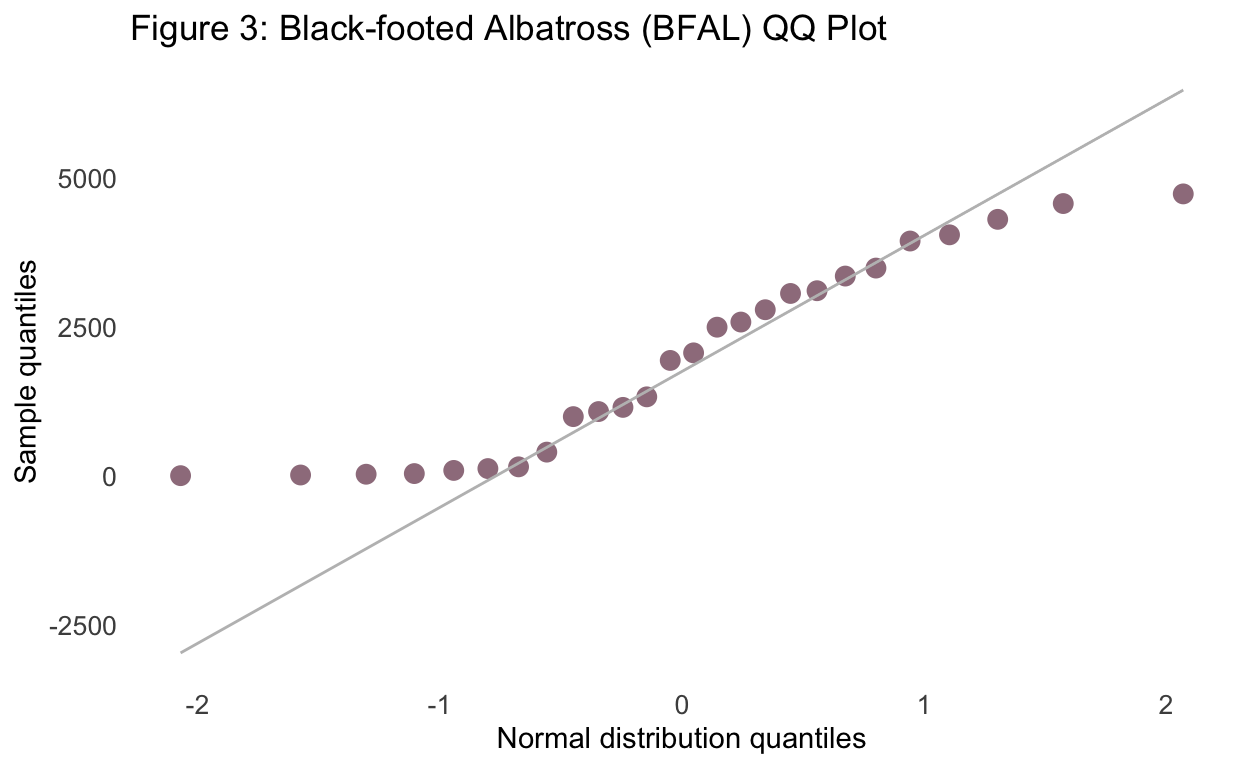
\includegraphics{hi_albatross_tokohu_tsunami_files/figure-latex/qqplot-1.pdf}

\begin{Shaded}
\begin{Highlighting}[]
\NormalTok{laal\_qqplot }\OtherTok{\textless{}{-}} \FunctionTok{ggplot}\NormalTok{(laal\_count) }\SpecialCharTok{+}
  \FunctionTok{geom\_qq}\NormalTok{(}\FunctionTok{aes}\NormalTok{(}\AttributeTok{sample =}\NormalTok{ total),}
          \AttributeTok{color =} \StringTok{"\#39ACB1"}\NormalTok{,}
          \AttributeTok{shape =} \DecValTok{17}\NormalTok{,}
          \AttributeTok{size =} \DecValTok{3}\NormalTok{) }\SpecialCharTok{+}
  \FunctionTok{geom\_qq\_line}\NormalTok{(}\FunctionTok{aes}\NormalTok{(}\AttributeTok{sample =}\NormalTok{ total),}
            \AttributeTok{color =} \StringTok{"grey"}\NormalTok{) }\SpecialCharTok{+}
  \FunctionTok{xlab}\NormalTok{(}\StringTok{"Normal distribution quantiles"}\NormalTok{) }\SpecialCharTok{+}
  \FunctionTok{ylab}\NormalTok{(}\StringTok{"Sample quantiles"}\NormalTok{) }\SpecialCharTok{+}
  \FunctionTok{labs}\NormalTok{(}\AttributeTok{title =} \StringTok{"Figure 4: Laysan Albatross (LAAL) QQ Plot"}\NormalTok{) }\SpecialCharTok{+}
  \FunctionTok{theme\_minimal}\NormalTok{() }\SpecialCharTok{+}
  \FunctionTok{theme}\NormalTok{(}\AttributeTok{line =} \FunctionTok{element\_blank}\NormalTok{(),}
        \AttributeTok{panel.grid =} \FunctionTok{element\_blank}\NormalTok{(),}
        \AttributeTok{strip.text =} \FunctionTok{element\_blank}\NormalTok{(),}
        \AttributeTok{axis.text.x =} \FunctionTok{element\_text}\NormalTok{(}\AttributeTok{size =} \DecValTok{10}\NormalTok{),}
        \AttributeTok{axis.text.y =} \FunctionTok{element\_text}\NormalTok{(}\AttributeTok{size =} \DecValTok{10}\NormalTok{),}
        \AttributeTok{legend.position =} \StringTok{"none"}\NormalTok{)}

\NormalTok{laal\_qqplot }
\end{Highlighting}
\end{Shaded}

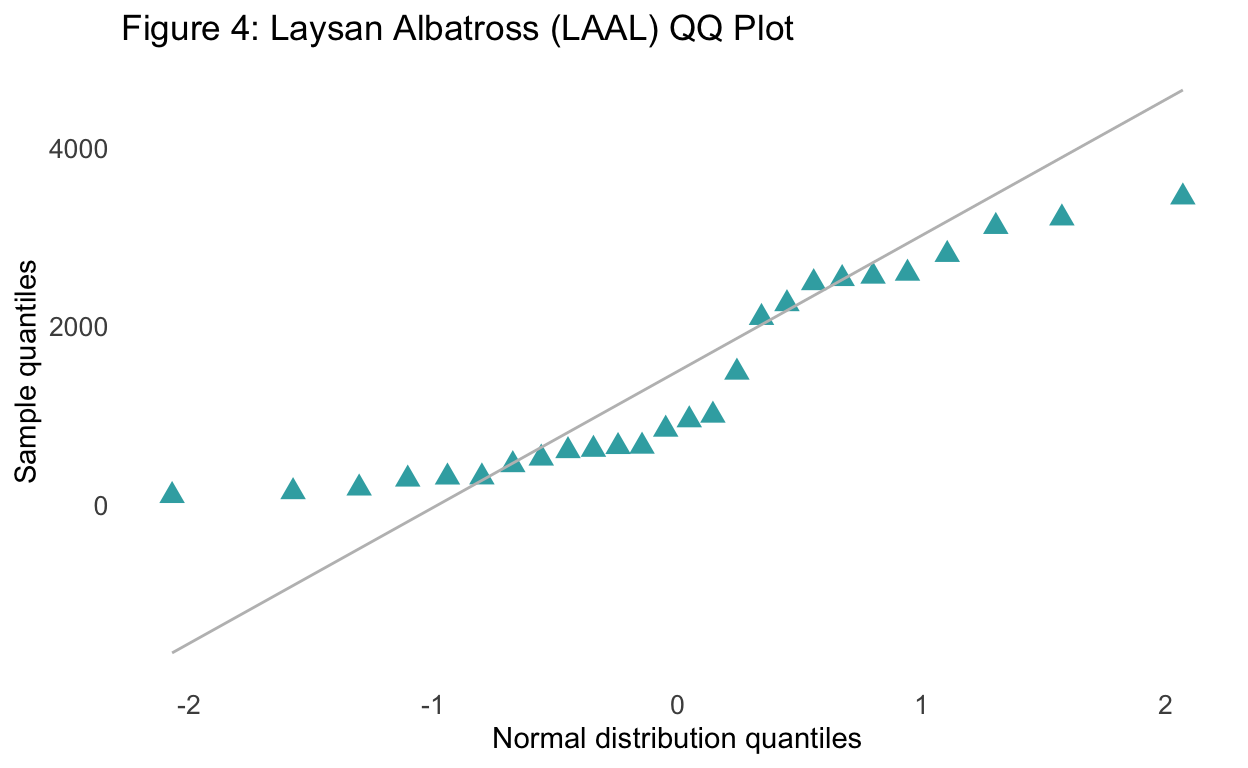
\includegraphics{hi_albatross_tokohu_tsunami_files/figure-latex/unnamed-chunk-18-1.pdf}

\hypertarget{simple-linear-regression}{%
\paragraph{Simple Linear Regression}\label{simple-linear-regression}}

The first regression I conducted on the albatross banding data was a
simple linear regression.

\[ \text{Albatross count}_i = \beta_0 + \beta_1 \text{tsunami event}  + \varepsilon_i \]

\begin{Shaded}
\begin{Highlighting}[]
\FunctionTok{tab\_model}\NormalTok{(post\_tsunami\_simple\_mod ,}
          \AttributeTok{pred.labels =} \FunctionTok{c}\NormalTok{(}\StringTok{"Intercept (mean albatross count pre{-}tsunami)"}\NormalTok{, }\StringTok{"Avg. banded albatross count post{-}tsunami"}\NormalTok{),}
          \AttributeTok{string.ci =} \StringTok{"Conf. Int (95\%)"}\NormalTok{,}
          \AttributeTok{string.p =} \StringTok{"P{-}value"}\NormalTok{,}
          \AttributeTok{title =} \StringTok{"Table 4: Simple Linear Regression Model for Banded Albatross in Hawaii"}\NormalTok{,}
          \AttributeTok{digits =} \DecValTok{4}\NormalTok{)}
\end{Highlighting}
\end{Shaded}

Table 4: Simple Linear Regression Model for Banded Albatross in Hawaii

~

total

Predictors

Estimates

Conf. Int (95\%)

P-value

Intercept (mean albatross count pre-tsunami)

2616.9667

2274.2624~--~2959.6710

\textless0.001

Avg. banded albatross count post-tsunami

-2169.0121

-2695.8899~--~-1642.1343

\textless0.001

Observations

52

R2 / R2 adjusted

0.578 / 0.569

The result of the simple regression shows that the intercept, 2616, is
the mean number of banded albatrosses in Hawaii prior to the Tōhoku
tsunami event in 2011. The second predictor, or \textbf{β1}, is the mean
banded albatrosses less than the intercept for any year after the
tsunami. For any year after the tsunami, the mean count is 447. There is
a 5\% chance that the average banded albatross will be between 2,2274
and 2,959 prior to the Tōhoku tsunami. The confidence interval
post-tsunami shows that the mean will be -2,695 and -1,642 of the total
albatrosses. Because the p-value is smaller than 0.05, the null
hypothesis that there was no impact from the Tōhoku tsunami on albatross
counts is rejected. The data provides convincing evidence that there is
a negative difference in mean number of albatrosses post-tsunami. There
is a statistically significant difference, at the 5\% significance
level, in the count of albatrosses in Hawaii. This model explains 57\%
of the variation in the albatross count data around its mean.

\hypertarget{multiple-linear-regression}{%
\paragraph{Multiple Linear
Regression}\label{multiple-linear-regression}}

The second regression I conducted on the albatross banding data was a
multiple linear regression with an interaction term of the tsunami event
on each albatross species.

\[ \text{Albatross count}_i = \beta_0 + \beta_1 \text{tsunami event} + \beta_2 \text{albatross species} + \beta_3\text{tsunami event:species} + \varepsilon_i \]

\begin{Shaded}
\begin{Highlighting}[]
\FunctionTok{tab\_model}\NormalTok{(interaction\_model,}
          \AttributeTok{pred.labels =} \FunctionTok{c}\NormalTok{(}\StringTok{"Intercept (mean BFAL count pre{-}tsunami)"}\NormalTok{, }\StringTok{"Mean BFAL count post{-}tsunami"}\NormalTok{, }\StringTok{"Mean LAAL count pre{-}tsunami"}\NormalTok{, }\StringTok{"Mean LAAL count compared to BFAL count post{-}tsunami"}\NormalTok{),}
          \AttributeTok{string.ci =} \StringTok{"Conf. Int (95\%)"}\NormalTok{,}
          \AttributeTok{string.p =} \StringTok{"P{-}value"}\NormalTok{,}
          \AttributeTok{title =} \StringTok{"Table 5: Multiple Linear Regression Model Results for Banded Albatross in Hawaii"}\NormalTok{,}
          \AttributeTok{digits =} \DecValTok{4}\NormalTok{)}
\end{Highlighting}
\end{Shaded}

Table 5: Multiple Linear Regression Model Results for Banded Albatross
in Hawaii

~

total

Predictors

Estimates

Conf. Int (95\%)

P-value

Intercept (mean BFAL count pre-tsunami)

3125.1333

2676.1144~--~3574.1523

\textless0.001

Mean BFAL count post-tsunami

-2653.4061

-3343.7333~--~-1963.0788

\textless0.001

Mean LAAL count pre-tsunami

-1016.3333

-1651.3420~--~-381.3246

0.002

Mean LAAL count compared to BFAL count post-tsunami

968.7879

-7.4823~--~1945.0580

0.052

Observations

52

R2 / R2 adjusted

0.653 / 0.631

The result of the simple regression shows that the intercept, 3125, is
the mean number of banded Black-footed albatrosses in Hawaii prior to
the Tōhoku tsunami event in 2011. The second predictor, or \textbf{β1},
is the mean banded Black-footed albatrosses less than the intercept for
any year after the tsunami. For any year after the tsunami, the mean
count is 472. The \textbf{β2} is the mean banded Laysan albatrosses less
than the mean number of Black-footed albatross before the tsunami. The
mean Laysan albatross count prior to the tsunami was 2,109. The
\textbf{β3} is the mean Laysan albatrosses count post-tsunami compared
to Black-footed albatrosses' post-tsunami. There are, on average, 969
more Laysan albatrosses than Black-footed albatrosses for any year after
the Tōhoku tsunami.

Since the p-values are smaller than 0.05, the null hypothesis that there
was no impact from the Tōhoku tsunami on albatross counts is rejected.
The data provides convincing evidence that there is a negative
difference in mean number of both Black-footed and Laysan albatrosses
post-tsunami. There is a statistically significant difference, at the
5\% significance level, in the count of albatross in Hawaii. The p-value
is greater than 0.05 when comparing the mean Laysan albatross count
post-tsunami to the Black-footed albatross. This predictor may indicate
that Laysan albatross counts were not as significantly impacted by the
tsunami as Black-footed albatross. This model explains 63\% of the
variation in the albatross count data around its mean.

\hypertarget{conclusion-and-future-research}{%
\subsection{Conclusion and Future
Research}\label{conclusion-and-future-research}}

In conclusion, the linear regression model predicts that there are
significant negative relationships between the independent variable
(years before and after tsunami) and the dependent variable (count of
banded albatross). It was also found that a multiple regression with an
interaction term based on the tsunami event impact of each albatross
species is a better model fit. This analysis indicates that the Tōhoku
tsunami had a negative impact on albatross populations in Hawaii.

For future analysis on the impact of the Tōhoku tsunami, I would like to
research what other variables may be influencing the number of
albatrosses being banded by biologist in Hawaii each year. I have a
suspension that there has been reduced banding effort throughout the
archipelago since the tsunami, especially in 2020 due to the pandemic. I
do not know why there would be a reduction in banding effort, but this
may be a significant influence on the count data used for this analysis.
I would also like to contact researchers in Hawaii to determine if there
is more comprehensive census data for albatross.

Two Black-footed albatross practicing their mating dances and calls,
while a Laysan albatross sits quietly on a nest in the background. The
Black-footed albatross on the right has been banded with two types of
bands (color and incoloy metal). The Black-footed albatross on the left
has not been banded. \emph{Image Credit: I. Nimz}

\hypertarget{corrections}{%
\subsection{Corrections}\label{corrections}}

If you see mistakes or want to suggest changes, please
\href{https://github.com/juliaparish/juliaparish.github.io/issues}{create
an issue} on the source repository.

\hypertarget{source-code}{%
\subsection{Source Code}\label{source-code}}

Find the source code for this blog post
\href{https://github.com/juliaparish/eds222_final}{here}.

\hypertarget{refs}{}
\begin{CSLReferences}{1}{0}
\leavevmode\vadjust pre{\hypertarget{ref-usfws:stal}{}}%
Alaska Region, U. S. Fish Wildlife Service -. n.d. {``Short-Tailed
Albatross (Phoebastria Albatrus).''}
\url{https://www.fws.gov/alaska/pages/endangered-species/short-tailed-albatross}.

\leavevmode\vadjust pre{\hypertarget{ref-Arata:2009}{}}%
Arata, Javier, Paul Sievert, and Maura Naughton. 2009. {``Status
Assessment of Laysan and Black-Footed Albatrosses, North Pacific Ocean,
1923-2005.''} \emph{U.S. Geological Survey Scientific Investigations
Report} 2009-5135: 80. \url{https://pubs.usgs.gov/sir/2009/5131/}.

\leavevmode\vadjust pre{\hypertarget{ref-iucn:2020}{}}%
List, IUCN Red. 2017. {``Black-Footed Albatross.''}
\url{https://www.iucnredlist.org/species/22698350/181896323}.

\leavevmode\vadjust pre{\hypertarget{ref-Reynolds:2017}{}}%
Reynolds, Michelle H., Paul Berkowitz, John Klavitter, and Karen
Courtot. 2017. {``Lessons from the Tōhoku Tsunami: A Model for Island
Avifauna Conservation Prioritization.''} \emph{Ecology and Evolution} 7
(15): 5873--90. \url{https://doi.org/10.1002/ece3.3092}.

\leavevmode\vadjust pre{\hypertarget{ref-plan:2012}{}}%
VanderWerf, Eric. 2012. {``Hawaiian Bird Conservation Action Plan.''}
\emph{Pacific Rim Conservation}.
\url{https://pacificrimconservation.org/wp-content/uploads/2013/10/Introduction\%202.pdf}.

\end{CSLReferences}

\end{document}
